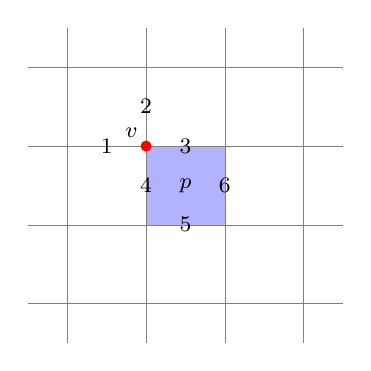
\begin{tikzpicture}[node font=\footnotesize]
  \draw [step=1, help lines]
    (-1.5,-1.5) grid (2.5,2.5);
  \draw [help lines, fill=blue!30]
    (0,0) rectangle (1,1) node [midway, black] {$p$};
  \fill [red]
    (0,1) node [above left, black] {$v$} circle (0.07);
  \draw
    (-0.5,1) node {$1$}
    ( 0,1.5) node {$2$}
    ( 0.5,1) node {$3$}
    ( 0,0.5) node {$4$}
    ( 0.5,0) node {$5$}
    ( 1,0.5) node {$6$};
\end{tikzpicture}
